\chapter{Background} 

\section{Complex Event Processing}
Complex Event Processing (CEP) ``is a defined set of tools and techniques for analyzing and controlling the complex series of interrelated events that drive modern distributed information systems.`` \citep{NpForMasses}. The Event Processing paradigm sees the world as a series of discrete events with the (producers) sources and sinks (consumers) of the events decoupled in space and time. In modern day distributed systems, events are delivered from sources to the sinks via an Infrastructure of distributed processors, which coordinate to provide processing and routing services. In such an Event based system, the sources and sinks may span a wide geographical area, connected by a CEP middleware, as described in \cite{Cugola}. The CEP middleware detects primitive events based on described patterns, interprets and combines them to identify higher level composite events. A CEP middleware thus can be said to be comprised of three key components:
\begin{itemize}
	\item  Rules Engine, responsible for expressing rules used by the compute node.
	\item  Compute Node, responsible for detecting primitive event patterns and interpreting them to generate complex events based on the rules.
	\item Notification Service, responsible for notifying the event sinks about the occurrence of events.
\end{itemize}
A CEP middleware is characterized by two important aspects: One, It decouples the source of the events from the sinks both in space and time; Two, it is capable of filtering events based on patterns and generating new events based on relationships among events using techniques of aggregation and composition. 
\begin{figure}[H]
	\centering
	\caption{Event Abstraction Hierarchy}
	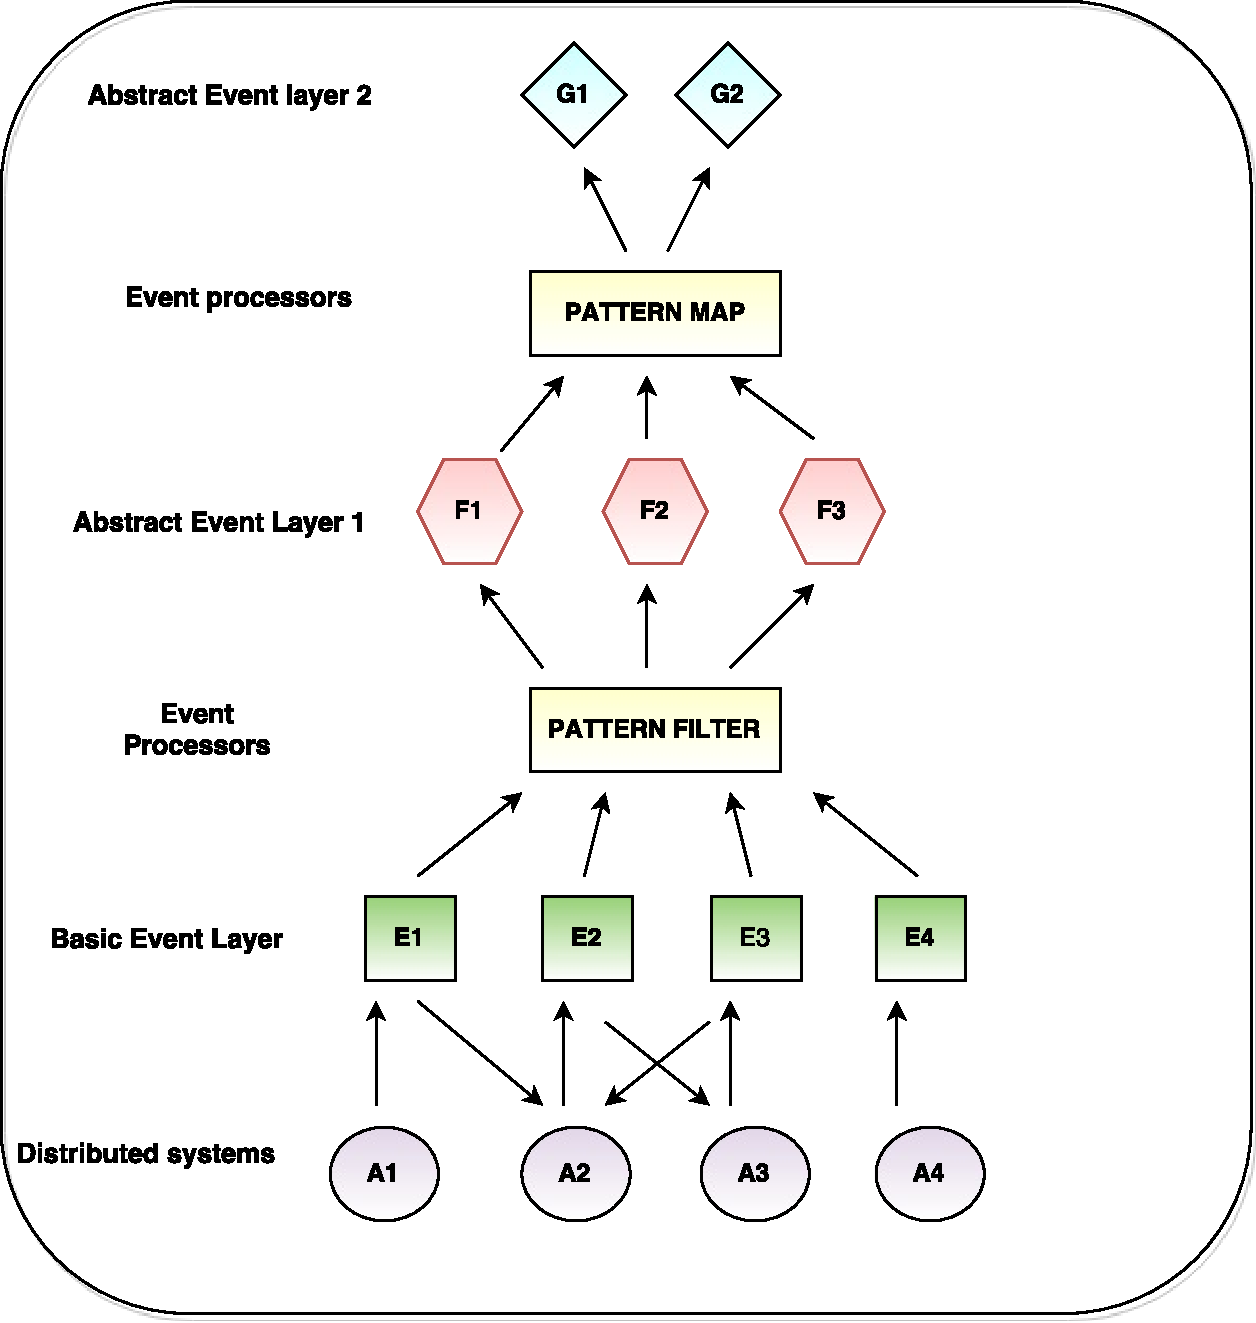
\includegraphics[height=10cm]{Luckham.pdf}
\end{figure}

\subsection{Hierarchical event abstraction}
Luckham et. al \cite{luckham1998complex} presents a hierarchical view of a complex event processing system based on a hierarchy of abstraction in events. As events move up the layer, they are subjected to different operations which transform the stream of events. At each layer of abstraction, the events may be delivered to interested sinks or sent to other compute nodes for further processing. A complex event processing system may thus be seen as series of operators applied to events depending on the desired event abstraction required by the consumers of events. Operator placement as such is a crucial research area in such systems. In section 3.1 a brief discussion is presented on the operator placement strategies within distributed complex event processing systems. 

\subsection{Communication models in complex event processing}
One of the most important traits of a complex event processing system is the decoupled nature of communication between the producer and consumer of events. 
\begin{itemize}
	\item Pub-Sub: In the publish-subscribe model of communication the senders of the message, otherwise called publishers, do not send the message to the receivers of the message, otherwise called subscribers. Rather the messages are published to a broker without the knowledge of the subscribers. The publishers advertise the topics to the broker and subscribers subscribe to a topic. A topic can have many publishers and many subscribers. On receiving a message on a topic, the brokers are responsible for delivering the message to the subscribers. Pub/Sub can be classified as a wide message delivery model of communication. Complex event processing systems are deployed using the pub-sub communication model for decoupled event delivery, where the consumers and producers of events are moving; with only the broker as a non-moving entity with compute nodes within complex event processing systems behaving both as producers and consumers of events. There are several Pub-Sub based notification services in the market today. Google Cloud Pub/Sub \cite{Krishnan2015} is one example of a thriving publish-subscribe message oriented middleware.
	
	\begin{figure}[H]
		\centering
		\caption{Publish-Subscribe communication model} 
		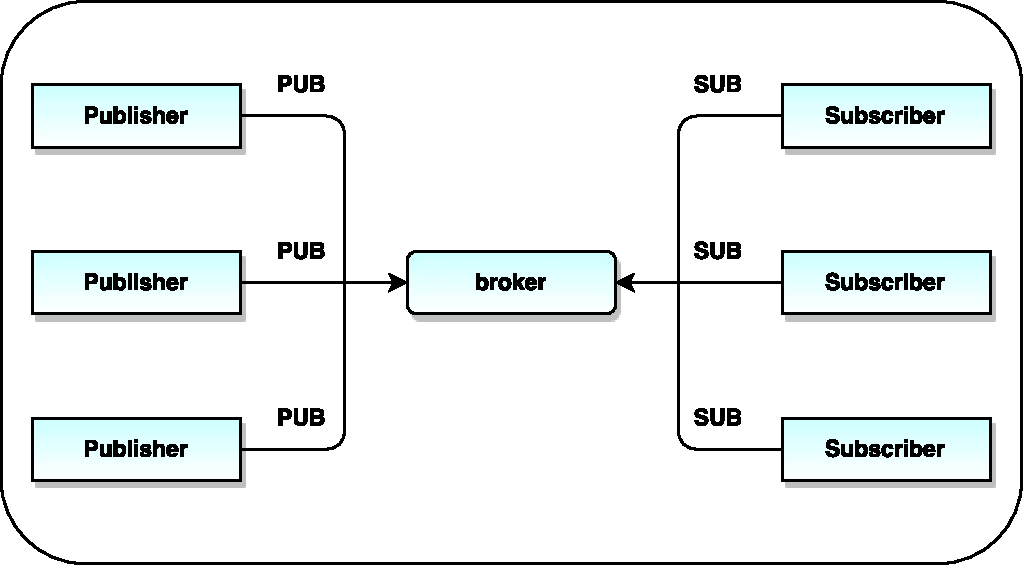
\includegraphics[height=6cm,width=12cm]{pubsub.pdf}
	\end{figure}
	\item Push-Pull: In a push-pull model of communication the messages are distributed to multiple workers who are registered as its pull clients. The pull clients which can do processing on their own do not rely on any broker but instead, have their pull clients to which the events are redirected. The extent of processing or filtering of events is directly dependent on the implementation. However, the events in this model of communication are sent evenly to multiple workers who may send the processed events to a single collector or different set of collectors create different stages of processing. The push-pull model is a pipe-lining pattern where all the subscribers need not receive the same message. Apache Kafka \cite{kafka2014high} is a high throughput distributed messaging system which uses the push-pull communication model to build robust data pipelines.
	
	\begin{figure}[H]
		\centering
		\caption{Push-Pull communication model} 
		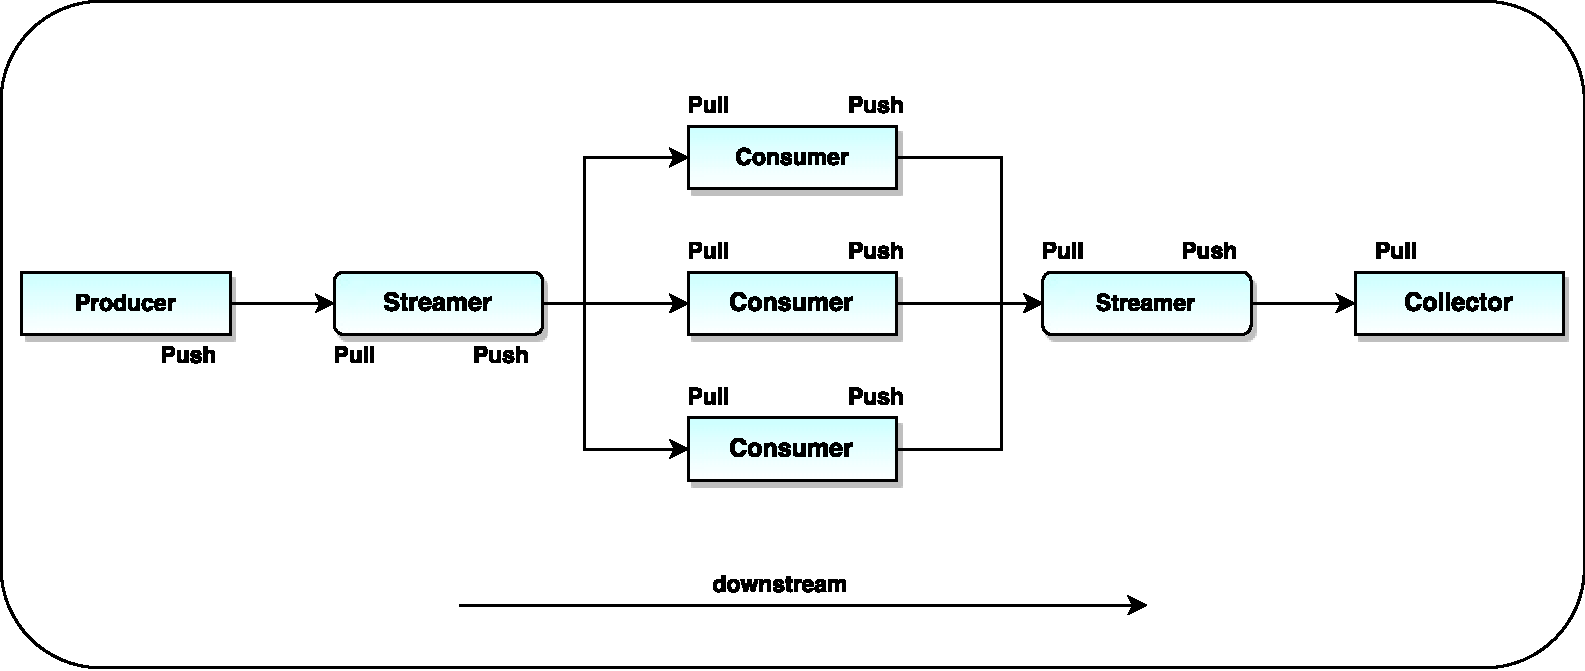
\includegraphics[height=8cm, width=16cm]{pushpull.pdf}
	\end{figure}
\end{itemize}


\subsection{Event Query languages}
Another crucial component of any complex event processing system is an event query language. Event query languages allow for the expression of user logic in a concise manner that is understood by the processing engine. Event query languages direct the processing engine to make sense of an event by describing the patterns for an event. Modern event query languages are equipped with capabilities to express temporal relationships among events with instructions for explicit and precise operations upon detection of events which share non-obvious relationships. Sophisticated features provided by modern event query languages include moving time windows, detection of causal relationships between events, aggregation of event data, generation of new events, etc. For example, Esper \cite{Esper} offers a domain specific language for dealing with high-frequency time-based events with SQL-like queries with support for sliding windows and event-series analysis.

\section{Software Defined Networking}
Software defined networking is a dynamic network programming paradigm that uses open interfaces to enable programmability of network devices. The primary focus is on aggregating the so-called control plane functionalities of all the network devices such as system configuration, management, and exchange of routing table information at a logically centralized location. The approach implies that the control path is decoupled from the fast path of the network device. While both the planes are set to evolve independently in a vendor agnostic manner, the fast path still utilizes the policy information made available by the control path to treat the packets both in the incoming and outgoing directions.\\\\The  figure 2.1 depicts a typical software defined network and provides the comparison with a legacy network. The devices in the traditional computer networks are comprised of both control plane and fast plane functionalities embedded into them directly as shown on the left-hand side of the diagram. Such devices lack the global network state information and require manual configuration during deployment. It also demands a certain mechanism to frequently propagate the routing information due to the distributed nature of the control plane.\\\\ The software defined network architecture, on the other hand, is built on top of the commercial off-the-shelf hardware components. The architecture is decomposed into three distinct layers of functionalities as shown on the right-hand side of the diagram.\\
\begin{itemize}
 \item Network infrastructure layer: It is the bottom most layer of the SDN ecosystem and contains the network devices themselves (both virtualized as well as physical devices) that are capable of switching/routing packets at line rate. They expose programmable interfaces to be leveraged by the upper layers of the SDN architecture.
 \item Controller layer: It is essentially the logically centralized control plane of the whole network infrastructure underneath. It forms the middle-ware of the SDN ecosystem and provides the necessary framework that binds the applications that require network services and the protocols that communicate with the network infrastructure. The vendor agnostic nature of the SDN architecture necessitates a set of communication mechanisms towards the network infrastructure which is commonly termed as southbound APIs. The OpenFlow, NETCONF, and OVSDB protocols are examples of such mechanisms provided by the SDN controller. 
 \item Application layer: The layer is composed of various network applications and the Northbound APIs exposed by the controller layer. Although there is no normative standard to describe what  Northbound APIs are comprised of, Restful APIs are prevalent in present day SDN applications. Some SDN controllers such as the OpenDayLight also provides OSGi based interfaces for native network application development.
\end{itemize}


\begin{figure}[H]
 \centering
 \caption{SDN Architecture}
 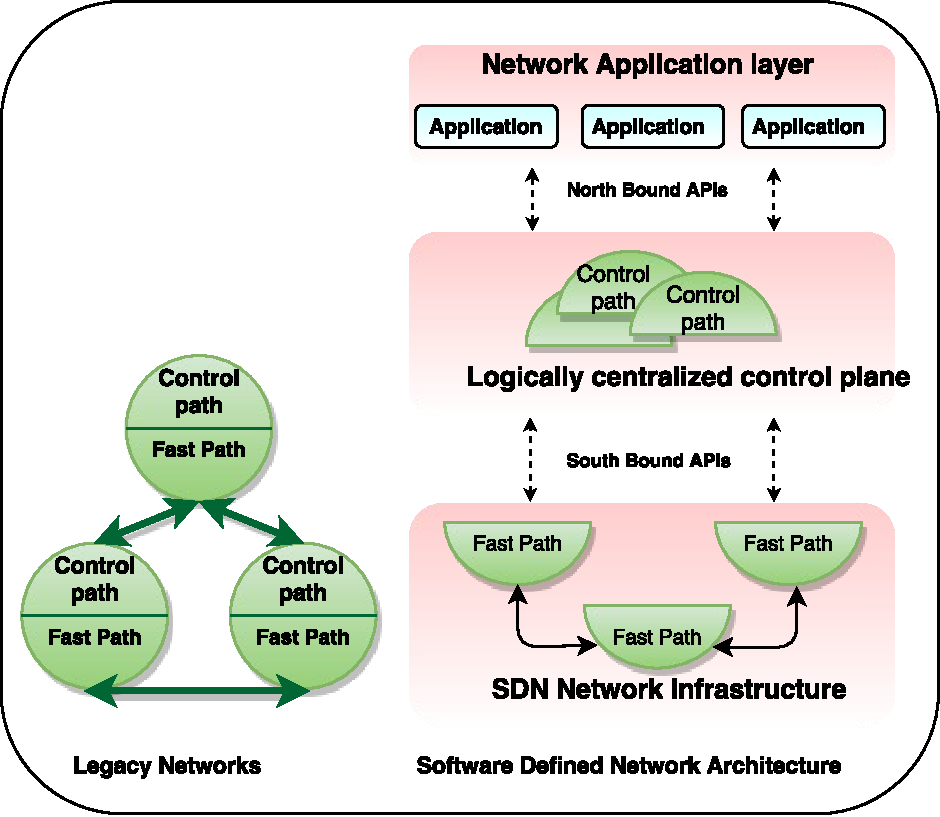
\includegraphics[height=10cm]{SDN-Architecture05.pdf}
\end{figure}

\section{OpenFlow}
The OpenFlow protocol is the default southbound API of choice in the SDN-enabled networks. Initially, it was considered as a communication mechanism that facilitates experimental protocols to be run in the computer networks \cite{OpenFlow-White-Paper}. It has now evolved into a rich set of APIs which can be leveraged to modify the forwarding behavior of network devices. The OpenFlow capable devices are manufactured from multiple vendors and include routers, switches, virtual switches, wireless access points\cite{OFArchive} and so on. \\\\To delve deep into the OpenFlow protocol features, the specification adheres to the SDN principle by separating control functions from the devices and thereby centrally managing the global forwarding policies in the network. The protocol has a set of messages defined for communication between the SDN controller and the underlying network. The OpenFlow capable switches operate based on the match-action policies programmed into their forwarding database. The match-action policies are defined on one or more flow-tables and a group table built into OpenFlow-capable switches. The flow-tables are essentially a set of rules containing packet headers/characteristics against which the packets in a flow are matched to make a packet modification/forwarding decision. The set of linked flow tables that provide matching, forwarding, and packet modification in an OpenFlow switch is termed as a pipeline \cite{OFSwitchSpecification} and hence the packets are said to undergo pipeline processing.  The pipeline processing of a packet may require that a packet traverses through one or all of the flow-tables defined in the incoming or outgoing direction. It should be noted that the packets are subjected to processing by a different set of flow-tables defined distinctly for ingress and egress directions. The SDN controller utilizes OpenFlow messages to add/modify/remove rules into and from the flow-tables.
The rules in a flow-table are assigned priorities to resolve match conflicts, and highest priority rule entry always takes effect, and the action(s) associated with the rule selected is executed. Besides actions, OpenFlow also allows several packet/byte level counters to be tagged along with a flow-rule. Such counters are useful in traffic monitoring, shaping and policing activities. The protocol, for the purpose mentioned above, also allows the SDN controller to describe a meter table with per flow meter entries (associated with flow rule entries) to achieve traffic shaping and policing. \\\\ Further, to provide an overview of the OpenFlow protocol communication mechanism, it supports three different type of messages:
\begin{itemize}
 \item Controller-to-switch: These messages are used to manage and obtain the status of the switches. For example, the controller can request a switch for its basic capabilities using the Features message.\\
 \item Asynchronous messages: These kinds of messages are triggered by the switches to inform the controller about change in operational status or other network events. For example, PACKET\_IN message is triggered to indicate a packet arrival event.\\
 \item Symmetric messages: These messages are typically heartbeat messages, error messages or initial Hello messages initiated by either of the parties i.e. the SDN controller or the network device. Some experimenter messages may also fall under this category.
\end{itemize}A detailed description of all the messages and their implied functionalities can be obtained from the OpenFlow specification document\cite{OFSwitchSpecification}. The OpenFlow protocol provides reliable message delivery through its channel connection built on top of TLS or simple TCP. The standard does not automatically impose any acknowledgments for the messages sent nor does it ensure ordered processing of messages and is left open for the switch implementations to handle the same.

\section{RYU SDN Controller}
SDN controller is the brain of the SDN ecosystem with all the network-wide control functions aggregated at the controller as a global snapshot which is then presented as a single logical switch to the application domain.  There have been several implementations of the controller since the inception of the SDN. Some of the salient features of an SDN controller include the ability to scale out the network without bounds, the ability to support network programming in a vendor agnostic manner, protocol agnostic characteristic that allows the design and use of new southbound APIs and so on.  Some of the open-sourced, adopted controllers are OpenDayLight, ONOS, Floodlight, RYU. As part of the thesis work, RYU is chosen as the controller for programming the Open vSwitch. RYU follows a simple modular design wherein applications are built and deployed as single threaded Python processes leveraging RYU's event based mechanism to interact with the other SDN applications. RYU also supports OpenFlow protocol along with various other southbound APIs which renders it just sufficient to extend the protocols, develop and deploy the desired controller application for this thesis work with a shorter development life cycle.\\\\RYU SDN controller at its core contains a set of components with well-defined APIs. The base component is the app\\manager which takes up the responsibilities such as loading RYU applications, providing contexts to RYU applications and routing messages between RYU applications. It has a dedicated OpenFlow controller component to handle protocol connections to the switches. The component also generates appropriate OpenFlow events to be handled by RYU applications. The other critical component of the controller is the RYU OpenFlow wire protocol encoder and decoder \cite{RYU-Documentation}.\\\\Each RYU application is equipped with its own FIFO message queue to receive events that are processed in the order of arrival. Although the application itself is expected to be developed as a single threaded module, RYU internally spawns a thread to handle events per application module. RYU provides another way to communicate with other applications/components by exchanging contexts which are essentially application specific python objects. Since the controller is built around event-based components, RYU applications naturally are equipped to observe and generate events. An application can observe/listen to events by using a specific python decorator exposed for event handling.\\\\ As part of the work, the OpenFlow protocol's match-action capability is extended to support event types and attributes. Through this mechanism, SDN controller facilitates the switches to detect events based on the event rules. The RYU controller like its counterparts also can provide Restful API support to network applications. The application developed hence exposes the Restful APIs to commission event-based rules on Open vSwitch.


\section{Intel Data Plane Development Kit}
Intel Data Plane Development Kit (DPDK) \cite{DPDK} is set of data plane libraries and userspace drivers that enable fast packet processing. Intel DPDK runs in Linux userspace and thus allows application programs to bypass the kernel for packet processing. As a consequence users of the DPDK libraries have the flexibility to run third-party fast path network stacks and develop fast packet capture algorithms all in the userspace. By enabling kernel bypass, DPDK reduces the number of cycles taken to send and receive packets. The main components of DPDK, as illustrated in the figure  are:

 \begin{figure}[H]
 \centering
 \caption{DPDK Components}
 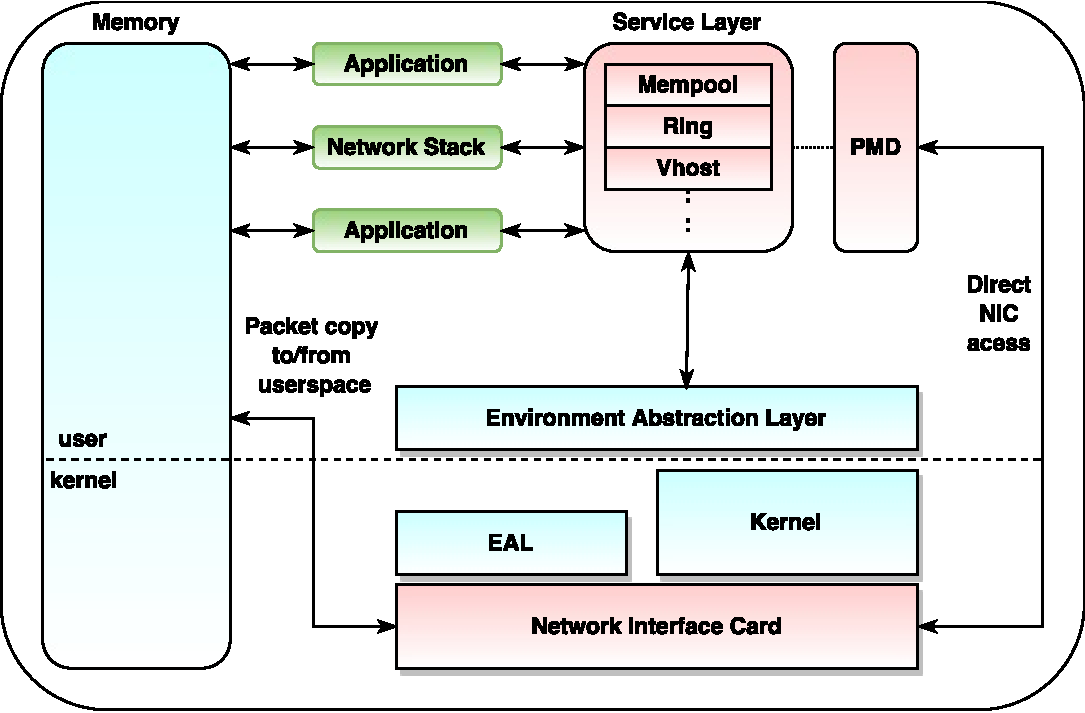
\includegraphics[height=9cm]{DPDK.pdf}
\end{figure}

\begin{itemize}
 \item Environment Abstraction Layer: The EAL provides an interface for the DPDK applications and libraries to access resources such as memory and hardware. The libraries and the applications are not aware of the allocation of these resources. The EAL is responsible for physical memory allocation, multi-process support, Interrupt-handling, PCI access, CPU feature recognition and core affinity setting among others.
 \item Service Layer: The service layer of DPDK consists of various libraries to enable DPDK applications to make use of the features provided by the EAL. The service layer can be seen as the provider of 'system calls' to the DPDK applications. For example, the ring library provides a lockless FIFO ring implementation for Rx and Tx queues with support for burst queue and dequeue; The Mempool library implements a pool-based aligned memory allocator with features such as per-core cache and hugepages; The vhost library provides a userspace virtio driver that allows the users to manipulate the vring. Full list of DPDK libraries can be found at \cite{DPDK}
 \item Poll Mode Drivers: The DPDK Poll Mode Drivers (PMD) provides userspace device drivers and APIS to set up queues and devices. The PMD is capable of accessing the transmit and receive queues directly without interrupts by continual polling. This ensures that the packets at the receive queues are directly received by the userspace application when receiving, and the packets from the user space are directly at transmit queues when sending.
\end{itemize}

\subsection{DPDK Vhost library}
The DPDK vhost library requires a special mention because of its support for vSwitch implementations. The vhost library provides a userspace vhost driver to manage vhost threads for corresponding virtio front-end devices in a guest. Before understanding the DPDK vhost library, it would be useful to understand the vhost-net acceleration standard on virtio. As illustrated in figure 1.1 in section 1.1, the Qemu userspace process normally provides the virtio back-end implementation for the virtio-net front-end device in a guest. This results in a situation where Qemu is involved intensely in the packet I/O thereby increasing the context switch required. As an improvement to this virtio standard of having a front-end in guest and back-end in Qemu, the vhost-net standard came into being. In the vhost-net implementation, a vhost-net device is introduced into the kernel space which acts as the back-end to the virtio front-end device in the guest. Keeping the vhost-net device in kernel ensures that Qemu process in not needed for every packet transfer between the host and guest. Instead, Qemu is involved in setting up the event file descriptors and the Interrupt file descriptors. Vhost creates an individual thread per virtio device which waits on the eventfd provided by Qemu. The host machine uses the eventfd to communicate with the guest by binding the eventfd to an interrupt source or listening to the eventfd which is triggered by the KVM when the guest writes the NOTIFY register. 

 \begin{figure}[H]
 \centering
 \caption{Vhost-net acceleration}
 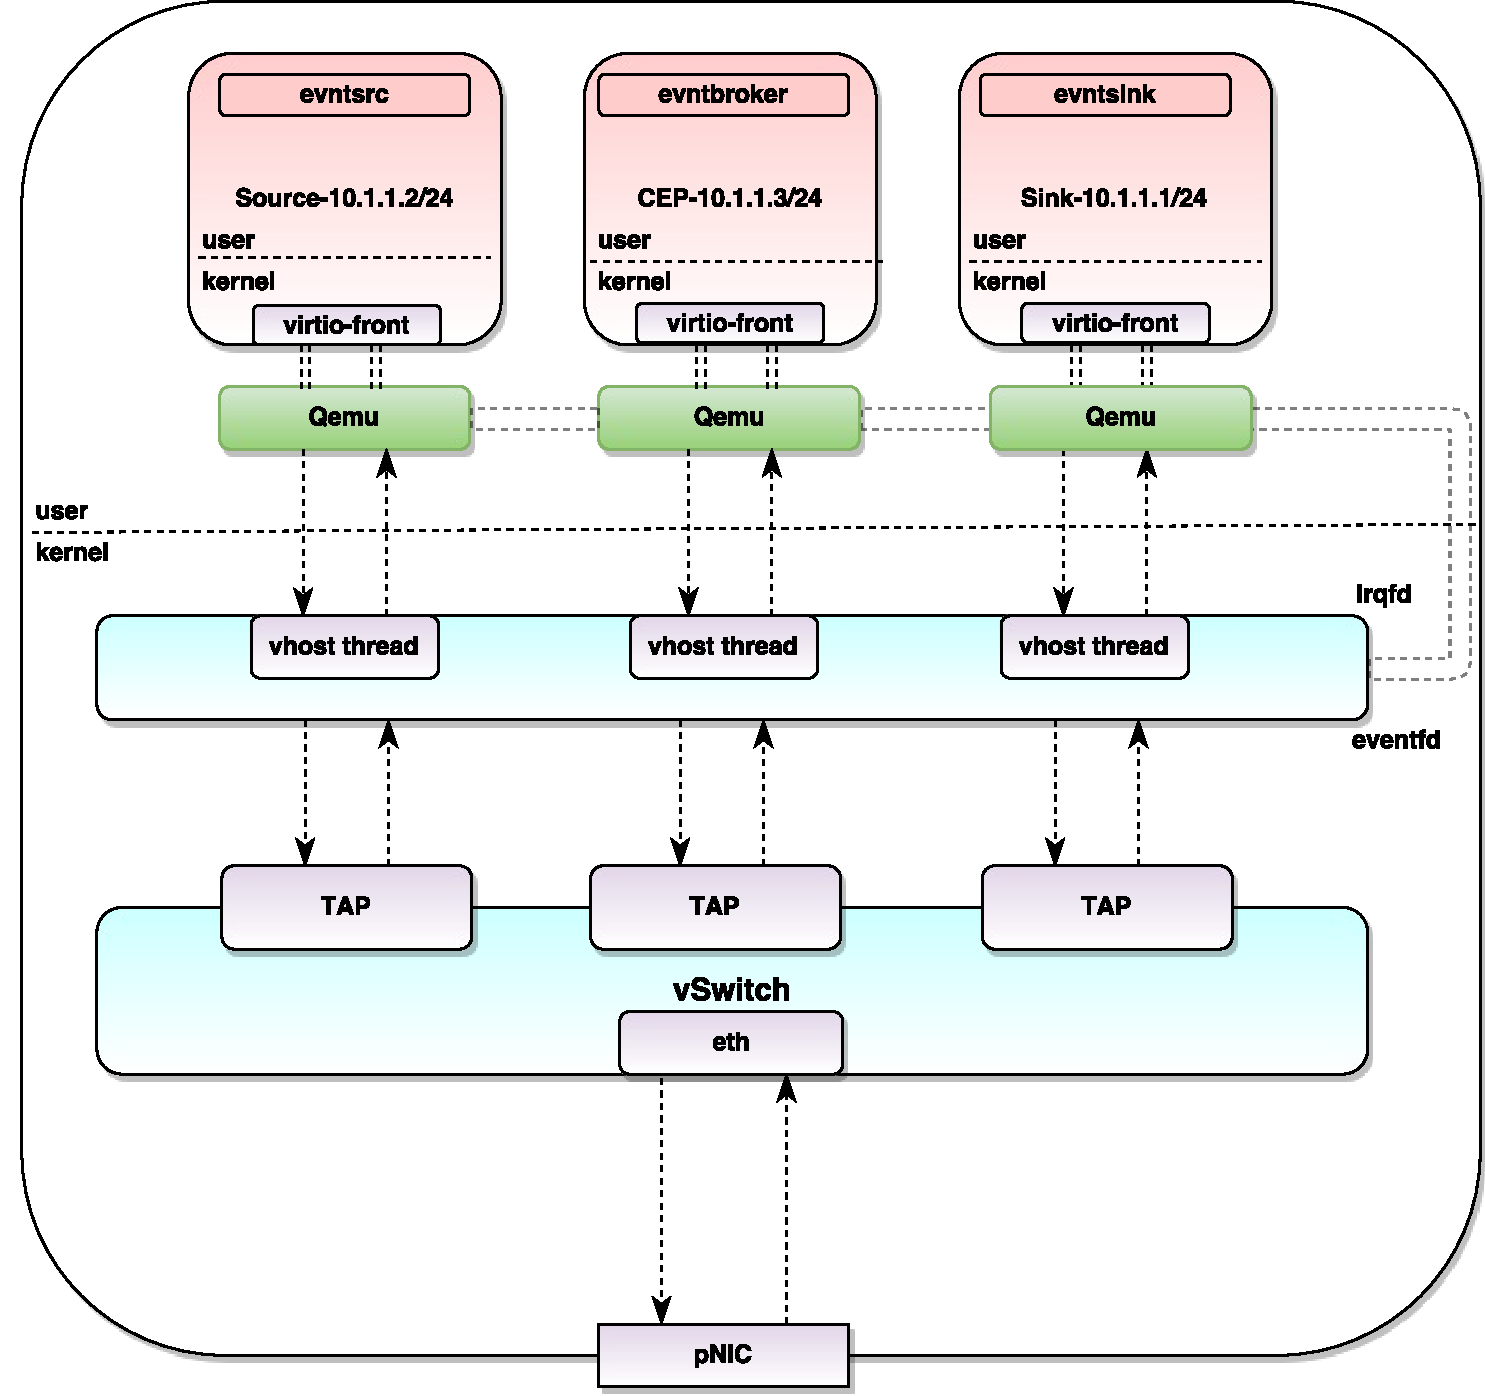
\includegraphics[height=12cm]{vhostnet.pdf}
\end{figure}

As illustrated in figure 2.5, vhost-net acceleration relies on Qemu for device feature negotiation, migration, etc. The vhost driver at the kernel is not a full-fledged virtio device implementation because Qemu still controls some parts of the setup. However, a virtqueue exists between the virtio-front end in the guest and Qemu. The vhost thread in the kernel can DMA to and from the virtqueue giving it access to the virtio-front end without Qemu intervention. This implementation can be contrasted with the DPDK vhost implementation which is illustrated in figure 5.13. In the DPDK vhost implementation, the vhost driver is moved completely to userspace. A dpdkvhostuser port attached to the vSwitch registers callbacks to the vhost library in userspace, which is called when the vhost device is activated/deactivated in the guest. For each virtio device in the guest, a vhost device is created by the vhost driver(vhost library). The dpdkvhostuser port (vhost-device) and the virtio device share a virtqueue that enables them to exchange packets without intervention from userspace Qemu directly. So a packet at the physical NIC is lifted into the userspace vSwitch where it is switched to the dpdkvhostuser port attached to the guest VM. Since the dpdkvhostuser port shares a virtqueue with the virtio device in the guest, the guest receives the packet with minimum overhead.
